\chapter{Lecture 34 - Laplace's Equation in Spherical Coordinates}
\label{ch:lec34}
\section{Objectives}
\begin{itemize}
\item Solve Laplace's equation in spherical coordinates. 
\item Introduce spherical harmonics.
\end{itemize}
\setcounter{lstannotation}{0}

\section{Boundary Value Problem}

In this lecture we will consider the problem of steady-state temperature in a sphere.  We will define our spherical coordinates as shown in Figure \ref{fig:lec34-spherical-coordinates}.  The relationship between $x$, $y$, $z$ and $r$, $\theta$, and $\phi$ are shown in the margin.
\begin{marginfigure}
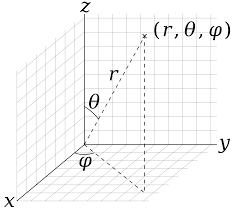
\includegraphics{lec34-spherical-coordinates.png}
\caption{Spherical coordinate system.}
\label{fig:lec34-spherical-coordinates}
\end{marginfigure}
\begin{margintable}
%\begin{table}
\begin{tabular}{l l}
$x = r\sin{\theta}\cos{\phi}$ & $0<r<c$ \\
$y = r\sin{\theta}\sin{\phi}$ & $0< \phi < 2\pi$ \\
$z = r\cos{\theta}$ & $0 < \theta < \pi$ \\
\end{tabular}
%end{table}
\end{margintable}

Laplace's equation could be stated generically enough as $\nabla^2u = 0$, of course, but we need to adapt the definition of the Laplacian operator for spherical coordinates.  This definition is shown in Equation \ref{eq:laplacian-spherical}.

\begin{equation}
\frac{\partial^2 u}{\partial r^2} + \frac{2}{r}\frac{\partial u}{\partial r} + \frac{1}{r^2 \sin{\theta}^2} \frac{\partial^2 u}{\partial \phi^2} + \frac{1}{r^2}\frac{\partial^2 u}{\partial \theta^2} + \frac{\cot{\theta}}{r^2}\frac{\partial u}{\partial \theta} = 0
\label{eq:laplacian-spherical}
\end{equation}

\noindent In order to make the complexity a little more manageable, we will assume a boundary condition that is only a function of $\theta$:
\begin{equation*}
u(c,\theta) = f(\theta)
\end{equation*}
Thus the solution will only be a function of $r$ and $\theta$ and all derivatives of $u$ with respect to $\phi$ can be eliminated from the Laplacian.  The governing equation will therefore be:
\begin{equation}
\frac{\partial^2 u}{\partial r^2} + \frac{2}{r}\frac{\partial u}{\partial r} + \frac{1}{r^2}\frac{\partial^2 u}{\partial \theta^2} + \frac{\cot{\theta}}{r^2}\frac{\partial u}{\partial \theta} = 0
\label{eq:lec34-ex1-ge}
\end{equation}
Despite all appearances, Equation \ref{eq:lec34-ex1-ge} is a linear, homogeneous, second-order boundary value problem so we will use separation of variables as usual.

\vspace{0.25cm}

\noindent\textbf{Step \#1:} Assume a product solution.
\begin{equation*}
u(r,\theta) = F(r)G(\theta)
\end{equation*}

\vspace{0.25cm}

\noindent\textbf{Step \#2:} Insert the product solution into the governing equation.
\begin{multline*}
\frac{\partial^2}{\partial r^2}\left[F(r)G(\theta)\right] + \frac{2}{r}\frac{\partial}{\partial r}\left[ F(r)G(\theta)\right] + \cdots \\
\frac{1}{r^2}\frac{\partial^2}{\partial \theta^2}\left[F(r)G(\theta)\right] + \frac{\cot{\theta}}{r^2}\frac{\partial}{\partial \theta}\left[F(r)G(\theta)\right] = 0 
\end{multline*}
\begin{align*}
F_{rr}G + \frac{2}{r}F_rG + \frac{1}{r^2}FG_{\theta \theta} + \frac{\cot{\theta}}{r^2}FG_{\theta} &= 0 \\
r^2F_{rr}G + 2rF_rG + FG_{\theta \theta} + \cot{\theta}FG_{\theta}&= 0
\end{align*}
\marginnote[-1.0cm]{Here we multiply through by $r^2$ to simplify the upcoming separation process.}

\vspace{0.25cm}

\noindent\textbf{Step \#3:} Separate the variables.

\begin{align*}
\frac{r^2 F_{rr}G}{FG} + \frac{2rF_rG}{FG} + \frac{FG_{\theta\theta}}{FG} + \frac{\cot{\theta}FG_{\theta}}{FG} &= 0 \\
\frac{r^2F_{rr}}{F} + \frac{2rF_r}{F} + \frac{G_{\theta\theta}}{G} + \frac{\cot{\theta}G_{\theta}}{G} &= 0 \\
\frac{r^2 F_{rr}}{F} + \frac{2rF_r}{F} = -\frac{G_{\theta\theta}}{G} - \frac{\cot{\theta}G_{\theta}}{G} &= \lambda
\end{align*}
So the separated equations are:
\begin{align*}
r^2F_{rr} + 2rF_{r} - \lambda F &= 0 \\
G_{\theta\theta} + \cot{\theta}G_{\theta} + \lambda G &= 0
\end{align*}
We can readily recognize the equation for $F(r)$ as a Cauchy-Euler equation.  But something badly needs to be done with the equation for $G(\theta)$.

\vspace{0.25cm}

\noindent\textbf{Step \#4:} Apply boundary conditions to determine non-trivial product solution(s).

\newthought{We will find}, eventually, that we can change the equation for $G(\theta)$ into something recognizable if we make the following transformation to the independent variable: $\cos{\theta} = x$.  Since $\theta$ goes from 0 to $\pi$ and $x = \cos{\theta}$, $x$ will go from -1 to 1. Let us set out on the process to replace all derivatives of $G$ with respect to $\theta$ to derivatives with respect to $x$. Using the chain rule:\marginnote[-0.0cm]{Here we use:
\begin{align*}
\frac{dx}{d\theta} &= -\sin{\theta} \\
&=-(1-x^2)^{\sfrac{1}{2}}
\end{align*}
An important detail here is that: $-\sin{\theta} = -(1-x^2)^{\sfrac{1}{2}}$ since $\cos{\theta}^2 + \sin{\theta}^2 = 1$ and therefore $\sin{\theta} = (1-cos{\theta}^2)^{\sfrac{1}{2}}$.}
\begin{align*}
G_{\theta} &= \frac{d}{dx}(G)\frac{dx}{d\theta} \\
&= -(1-x^2)^{\sfrac{1}{2}}G_x
\end{align*}

Repeating to find an expression for $G_{\theta\theta}$:
\begin{align*}
G_{\theta \theta} &= \frac{d}{dx}(G_{\theta})\frac{dx}{d\theta} \\
&=\frac{d}{dx}\left[-(1-x^2)^{\sfrac{1}{2}}G_x\right]\left[-(1-x^2)^{\sfrac{1}{2}}\right] \\
&=\left[-\frac{1}{2}(1-x^2)^{-\sfrac{1}{2}}(-2x)G_x - (1-x^2)^{\sfrac{1}{2}}G_{xx}\right]\left[-(1-x^2)^{\sfrac{1}{2}}\right] \\
&=\frac{1}{2}(-2x)G_x + (1+x^2)G_{xx}
\end{align*}
Inserting these expressions into our equation for $G(\theta)$ gives us:
\begin{equation*}
\overbrace{-xG_{x}+(1-x^2)G_{xx}}^{G_{\theta \theta}} + \underbrace{\frac{x}{1-x^2}^{\sfrac{1}{2}}}_{\substack{\cot{\theta} \\ \\ = \frac{\cos{\theta}}{\sin{\theta}}}}\overbrace{\left[-1(1-x^2)^{\sfrac{1}{2}}G_x \right]}^{G_{\theta}} + \lambda G = 0
\end{equation*}
which, upon simplification is:
\begin{equation*}
(1-x^2)G_{xx} - 2xG_x + \lambda G = 0
\end{equation*}
Which is, at long last, Legendre's equation.  Recall that Legendre's equation has polynomial solutions for $\lambda = n(n+1), \ n=0,1,2,\dots$ and these solutions are called Legendre polynomials, $P_n(x)$. Substituting now $x = \cos{\theta}$, we get the solution for $G(\theta)$:
\begin{equation*}
G(\theta) = c_1P_n(\cos{\theta})
\end{equation*}
The functions $P_n(\cos{\theta})$ are sometimes called \emph{spherical harmonics}.\marginnote{Functions that are solutions to Laplace's equation are called \emph{harmonics}.  Spherical harmonics solve Laplace's equation in spherical coordinates.}

\newthought{Now that we} have solutions for $G(\theta)$ as well as our allowed eigenvalues, we circle back to solve $F(r)$.  Following the usual procedure for Cauchy-Euler equations, we assume a solution of the form $F(r)=r^m$ and find values of $m$ that satisfy the equation:
\begin{align*}
r^2F_{rr} + 2rF_r - n(n+1)F &= 0 \\
r^2\left[m(m-1)r^{m-2}\right]+2rmr^{m-1}-n(n+1r^m &= 0 \\
r^m\left[m^2-m+2m-n(n+1) \right] &= 0 \\
m^2+m-n(n+1) &= 0 \\
(m-n)(m+(n+1)) &= 0 \\
\Rightarrow m = n, -(n+1)
\end{align*}
Therefore the general solution for $F(r)$ is:
\begin{equation*}
F(r) = c_2r^n + c_3r^{-(n+1)}
\end{equation*}
In order to ensure that $\lim_{r \to 0} F(r)<\infty$, we must set $c_3 = 0$.  The product solution is given in Equation \ref{eq:lec34-ex-sol}.\marginnote[-1.5cm]{Admittedly, this is the only boundary condition that we have applied so far for this problem. We latched on to the eigenvalues $\lambda = n(n+1)$, for non-negative integer $n$, and did not explore what would happen if $n$ is negative.  In the interest of time and space in this lecture, I ask that we leave well-enough alone and leave that exploration for another day.} 
\begin{equation}
u(r,\theta) = \sum\limits_{n=0}^{\infty} c_n r^nP_n(cos{\theta})
\label{eq:lec34-ex-sol}
\end{equation}

\vspace{0.25cm}

\noindent\textbf{Step \#5:} Apply the remaining boundary conditions to determine the unknown coefficients.

\vspace{0.25cm}

\noindent The last boundary condition we have to apply is on the outside surface of the sphere:
\begin{equation*}
u(R,\theta) = \sum\limits_{n=0}^{\infty}c_n R^n P_n(\cos{\theta}) = f(\theta)
\end{equation*}
On the left of the last equality we have an infinite linear combination of orthogonal functions; on the right we have a function.  We want to know the values of $c_n$ so that they will be equal.  How do we do this?  We multiply both sides by an orthogonal function, and weight function, and integrate.

\newthought{This case is} a bit different than the last time we met Legendre polynomials, however, insofar as the argument for $P_n$ is now $\cos{\theta}$ and not $x$.  Suppose we pretended, temporarily, that we were dealing with $P_n(x)$; what would we do?  The equation for $c_n$ would look something like:
\begin{align*}
\int_{-1}^{1}c_n R^n P_n(x)^2 \ dx &= \int_{-1}^{1} f(x) P_n(x) \ dx \\
\Rightarrow c_n &= \frac{1}{R^n}\frac{\int_{-1}^{1} f(x) P_n(x) \ dx}{\int_{-1}^{1} P_n(x)^2 \ dx}
\end{align*}
But in our case, we have $P_n(\cos{\theta})$; we need to change variables, again, to reflect $x = \cos{\theta}$, and $dx = -\sin{\theta} \ d\theta$.  We must also make substitutions in the limits of integration: if $x=\cos{\theta}$, when $x=-1$, $\theta = \pi$;  also $x=\cos{\theta}$ when $x=1$, corresponds to $\theta = 0$.  Making these substitutions into our expression gives us the formula for our coefficients in Equation \ref{eq:lec34-ex-coeff}.\marginnote[-1.0cm]{With the given substitutions, the formulat for $c_n$ becomes:

$$c_n = \frac{\int_{\pi}^0 f(\theta)P_n(\cos{\theta}(-\sin{\theta}) \ d\theta}{R^n \int_{\pi}^{0} P_n(\cos{\theta})^2 \ (-\sin{\theta}) \ d\theta}  $$

\noindent In Equation \ref{eq:lec34-ex-coeff} we flipped the bounds of integration and removed the minus sign from $(-\sin{\theta})$.}
\begin{equation}
c_n = \frac{\int_{0}^{\pi} f(\theta) P_n(\cos{\theta}) \sin{\theta} \ d\theta}{R^n\int_{0}^{\pi} P_n(\cos{\theta})^2 \sin{\theta} \ d\theta}
\label{eq:lec34-ex-coeff}
\end{equation}

\section{MATLAB Implementation}
In the code listings below we will construct the solution for $R = 2$ and $f(\theta)$ given by:
\begin{equation*}
f(\theta) = 
\begin{cases}
10(\sfrac{\pi}{2}-\theta), & 0 \le \theta < \sfrac{\pi}{2} \\
0, & \sfrac{\pi}{2} \le \theta \le \pi
\end{cases}
\end{equation*}
We start, as usual, by clearing out the workspace and setting problem parameters.
\begin{lstlisting}[name=lec34-ex, style=myMatlab]
clear
clc
close 'all'
%% Set Parameters
R = 2;
N = 4;
f = @(theta) ex1(theta);
\end{lstlisting}
Next we construct the solution for the specified number of eigenfunctions.
\begin{lstlisting}[name=lec34-ex, style=myMatlab]
%% Construct the Solution
c = nan(N,1);
u = @(r,theta) 0; % initialize the series

% start for n = 0 
n = 0;
c0 = integral(@(th) f(th).*...
    legendreP(n,cos(th)).*sin(th),0,pi)./...
    integral(@(th) (R^n)*...
    (legendreP(n,cos(th)).^2).*sin(th),0,pi);

u = @(r,theta) u(r,theta) + c0*(r.^0).*legendreP(n,cos(theta));    

for n = 1:N 
    % get the next coeficient
    c(n) = integral(@(th) f(th).*...
        legendreP(n,cos(th)).*sin(th),0,pi)./...
        integral(@(th) (R^n)*...
        (legendreP(n,cos(th)).^2).*sin(th),0,pi);
    
    % update the approximation
    u = @(r,theta) u(r,theta) + ...
        c(n)*(r.^n).*legendreP(n,cos(theta)); 
end
\end{lstlisting}
Next we would like to visualize the results.  At the time of this writing, MATLAB has limited capability for visualizing three-dimensional data.  For the example, we will tabulate the solution on a regular mesh comprising a cube that contains the sphere of interest.  The tabulated solution will be written to a VTK\sidenote{VTK stands for ``Visualization Toolkit'' and a VTK data file is one of several standard data formats used for storing scientific data as it is prepared for visualization.} data file that can be visualized with software tools such as ParaView.\cite{paraview}
\begin{lstlisting}[name=lec34-ex, style=myMatlab]
%% Process Result for Plotting 
Nx = 50;
Xv = linspace(-R,R,Nx);
Yv = linspace(-R,R,Nx);
Zv = linspace(-R,R,Nx);
dx = Xv(2)-Xv(1); % need this for VTK file
[XX,YY,ZZ] = meshgrid(Xv,Yv,Zv);

RR = sqrt(XX.^2+YY.^2+ZZ.^2);
PP = acos(ZZ./RR);
UU = u(RR,PP); 
% set region outside the sphere to nan
UU(RR>R) = nan;

%% Write the data to a file
filename = 'solution.vtk';
dataname = 'U';
origin = [-R -R -R]; 
spacing = [dx dx dx];
save_scalarStructuredPoints3D_VTK_binary(filename,...
    dataname,UU,origin,spacing);
\end{lstlisting}
Lastly, let us show the local functions used to represent the boundary condition and to write the resulting data into a properly formatted VTK file.
\marginnote[4.0cm]{
\ref{lst:ann34-1-1} This local function, as the name suggests, saves the scalar data---which is organized in a three-dimensional regular grid---into a binary data file.  The ASCII file header is a specified format and is used to describe the structure of the data so that software like ParaView can be used to visualize the data.  We refer to this as a ``binary data file'' since the actual data is stored in binary form.  Alternatively the data could be stored in plain text but that would make the file much larger.
}
\begin{lstlisting}[name=lec34-ex, style=myMatlab]
%% Local functions
function u = ex1(theta)
[n,m] = size(theta);
u = nan(n,m);
ind_a = theta<=(pi/2);
ind_b = theta>(pi/2);
u(ind_a) = 10*((pi/2)-theta(ind_a));
u(ind_b) = 0;
end

function save_scalarStructuredPoints3D_VTK_binary(filename,... /*!\annotation{lst:ann34-1-1}!*/
    dataname,data_set,origin,spacing)

[nx,ny,nz]=size(data_set);

% open the file
fid = fopen(filename,'w');

% ASCII file header
fprintf(fid,'# vtk DataFile Version 3.0\n');
fprintf(fid,'VTK from Matlab\n');
fprintf(fid,'BINARY\n\n');
fprintf(fid,'DATASET STRUCTURED_POINTS\n');
fprintf(fid,'DIMENSIONS %d %d %d \n',nx,ny,nz);
fprintf(fid,'ORIGIN  %4.3f   %4.3f  %4.3f \n',...
    origin(1),origin(2),origin(3));
fprintf(fid,'SPACING %4.3f   %4.3f  %4.3f \n',...
    spacing(1),spacing(2),spacing(3));
fprintf(fid,'\n');
fprintf(fid,'POINT_DATA %d \n',nx*ny*nz);
fprintf(fid,strcat('SCALARS','\t ',dataname,' float ', '\n'));
fprintf(fid,'LOOKUP_TABLE default \n');
% write the data
fwrite(fid,reshape(data_set,1,nx*ny*nz),'float','b');
% close the file
fclose(fid);

end

\end{lstlisting}
The solution for this case is shown in Figure \ref{fig:lec34-ex-plot}.
\begin{marginfigure}
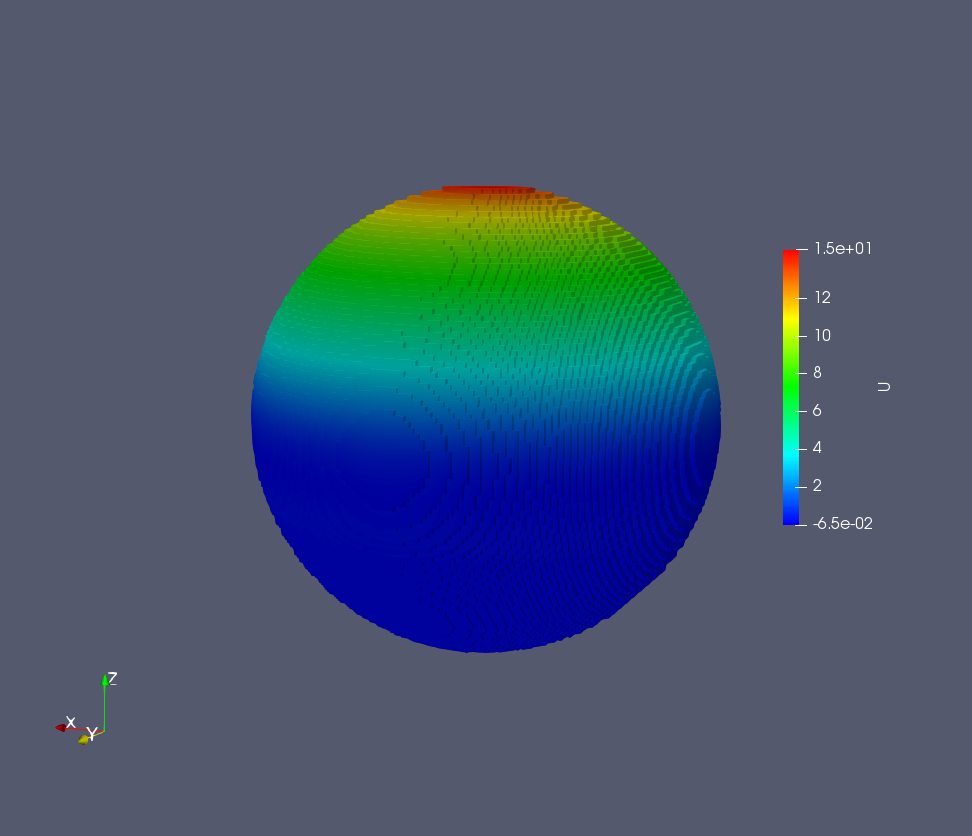
\includegraphics{lec34-ex-plot.png}
\caption{Plot of solution using ParaView.}
\label{fig:lec34-ex-plot}
\end{marginfigure}

